

%------------------------------------------------------------------------------
\subsection{The $P_1\times P_0$ pair} \label{ss:p1p0}
\index{general}{$P_1\times P_0$}
%---
example 3.70 in \textcite{john16} (book),


Elman Silvester Wathen say (5.3.3) that 
``it can be readily stabilized using the pressure jump
stabilization together with an appropriate macroelement subdivision.''
See \textcite{nosi98} (1998) for globally and locally stabilised versions. 

\textcite{qizh07b} (2007) states: ``the element is unstable for any mesh since
the dimension of the discrete velocity space is always less than that of the pressure space (with
Dirichlet boundary condition).'' The authors explain a filter algorithm to make the
element usable. 

\textcite{arno93} (1993) states: ''Unfortunately, this simplest possible Stokes element is notoriously unstable. On any tri-
angulation with at least three vertices on the boundary the dimension of the pressure
space exceeds that of the velocity space [...] and the finite
dimensional problem is singular. 
Moreover, while the discrete velocity field $u_h$ is uniquely
determined (as it is for any conforming method for the Stokes problem), for this choice of
elements $u_h$ belongs to the space of divergence-free fields piecewise linear fields, and on
many meshes, for example on a uniform diagonal mesh of the square [...],
this space is known to reduce to zero. So even after accounting for the indeterminancy of
the pressure we have no convergence.''

Example 3.2 of \textcite{bobf08} (2008) explains neatly the locking phenomenon and how 
to circumvent it via a so-called cross-grid macroelement. See also 
\textcite{hokl03} (2003).

In his lecture notes\footnote{\url{https://www.math.tamu.edu/~guermond/}}, 
Guermond states ``A simple alternative to the 
$Q_1\times P_0$ element consists of using the $P_1\times P_0$ element.
Let ${\cal T}_h$  be a mesh of $D$ composed of affine simplices, and approximate the 
velocity with continuous piecewise linear polynomials and the pressure with
(discontinuous) piecewise constants. Since the velocity is piecewise linear, its
divergence is constant on each simplex. As a result, testing the divergence
of the velocity with piecewise constants enforces the divergence to be zero
everywhere. That is to say, the $P_1\times P_0$ finite element yields a velocity 
approximation that is exactly divergence-free [...]. Unfortunately,
this pair does not satisfy the inf-sup condition.''

I have not found a paper yet which showcases its accuracy on a manufactured solution
and compares it to other element pairs.




%------------------------------------------------------------------------------
\subsection{The $P_1^+\times P_0$ pair} \label{ss:p1pp0}
\index{general}{$P_1^+\times P_0$}
\begin{flushright} {\tiny {\color{gray} pair\_p1pp0.tex}} \end{flushright}
%~~~~~~~~~~~~~~~~~~~~~~~~~~~~~~~~~~~~~~~~~~~~~~~~~~~~~~~~~~~~~~~~~~~~~~~~~~~~~~~~~~~~~~~~~~~~~~~~~~

\begin{center}
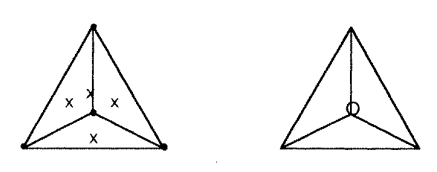
\includegraphics[width=6cm]{images/pair_p1pp0/p1pp0}\\
{\captionfont Taken from \textcite{begt92} (1992).}
\end{center}

In Table I of \textcite{begt92} (1992) we find:
\begin{eqnarray}
\bN_1(r,s,t) &=& (1-r-s-t)-\frac13 (\bN_5+\bN_6+\bN_7) \qquad \vec{r}_1=(0,0,0) \nn\\
\bN_2(r,s,t) &=& r-\frac13 (\bN_5+\bN_6+\bN_8)         \qquad \vec{r}_2=(1,0,0) \nn\\
\bN_3(r,s,t) &=& s-\frac13 (\bN_5+\bN_7+\bN_8)         \qquad \vec{r}_3=(0,1,0) \nn\\
\bN_4(r,s,t) &=& t-\frac13 (\bN_6+\bN_7+\bN_8)         \qquad \vec{r}_4=(0,0,1) \nn\\
\bN_5(r,s,t) &=& 27(1-r-s-t)rs          \qquad \vec{r}_5=(\frac13,\frac13,0) \nn\\
\bN_6(r,s,t) &=& 27(1-r-s-t)rt          \qquad \vec{r}_6=(\frac13,0,\frac13) \nn\\
\bN_7(r,s,t) &=& 27(1-r-s-t)st          \qquad \vec{r}_7=(0,\frac13,\frac13) \nn\\
\bN_8(r,s,t) &=& 27rst  \qquad\qquad\qquad\quad \vec{r}_8=(\frac13,\frac13,\frac13) 
\end{eqnarray}
Note that we can verify that
\begin{eqnarray}
\sum_{i=1}^8 \bN_i(r,s,t) 
&=& \bN_1 +\bN_2 +\bN_3 +\bN_4 +\bN_5 +\bN_6 +\bN_7 +\bN_8 \nn\\
&=& (1-r-s-t)-\frac13 (\bN_5+\bN_6+\bN7) \nn\\
&+& r-\frac13 (\bN_5+\bN_6+\bN8)  
 +  s-\frac13 (\bN_5+\bN_7+\bN8) 
 +  t-\frac13 (\bN_6+\bN_7+\bN8) \nn\\
&+& \bN_5 + \bN_6 + \bN_7 + \bN_8  \nn\\
&=& 1
+(-\frac13 -\frac13 -\frac13+1)\bN_5
+(-\frac13 -\frac13 -\frac13+1)\bN_6
+(-\frac13 -\frac13 -\frac13+1)\bN_7
+(-\frac13 -\frac13 -\frac13+1)\bN_8 \nn\\
&=& 1
\end{eqnarray}





%------------------------------------------------------------------------------
\subsection{The ${ P}_1^{++}\times P_{-1}$ pair} \label{ss:p1ppp1}
\begin{flushright} {\tiny {\color{gray} pair\_p1ppp10.tex}} \end{flushright}
%~~~~~~~~~~~~~~~~~~~~~~~~~~~~~~~~~~~~~~~~~~~~~~~~~~~~~~~~~~~~~~~~~~~~~~~~~~~~~~~~~~~~~~~~~~~~~~~~~~


\begin{center}
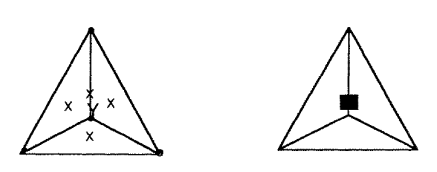
\includegraphics[width=6cm]{images/pair_p1ppp1/p1ppp1}\\
{\captionfont Taken from \textcite{begt92} (1992).}
\end{center}

In Table I of \textcite{begt92} (1992) we find:
\begin{eqnarray}
\bN_1(r,s,t) &=& (1-r-s-t)-\frac13 (\bN_5+\bN_6+\bN_7)-\frac14 \bN_9 \qquad \vec{r}_1=(0,0,0) \nn\\
\bN_2(r,s,t) &=& r-\frac13 (\bN_5+\bN_6+\bN_8)-\frac14 \bN_9 \qquad \vec{r}_2=(1,0,0) \nn\\
\bN_3(r,s,t) &=& s-\frac13 (\bN_5+\bN_7+\bN_8)-\frac14 \bN_9 \qquad \vec{r}_3=(0,1,0) \nn\\
\bN_4(r,s,t) &=& t-\frac13 (\bN_6+\bN_7+\bN_8)-\frac14 \bN_9 \qquad \vec{r}_4=(0,0,1) \nn\\
\bN_5(r,s,t) &=& 27(1-r-s-t)rs-\frac{108}{256}\bN_9          \qquad \vec{r}_5=(\frac13,\frac13,0) \nn\\
\bN_6(r,s,t) &=& 27(1-r-s-t)rt-\frac{108}{256}\bN_9          \qquad \vec{r}_6=(\frac13,0,\frac13) \nn\\
\bN_7(r,s,t) &=& 27(1-r-s-t)st-\frac{108}{256}\bN_9          \qquad \vec{r}_7=(0,\frac13,\frac13) \nn\\
\bN_8(r,s,t) &=& 27rst-\frac{108}{256}\bN_9  \qquad\qquad\qquad\quad \vec{r}_8=(\frac13,\frac13,\frac13)\nn\\ 
\bN_9(r,s,t) &=& 256(1-r-s-t)rst \qquad\qquad\qquad \vec{r}_9=(\frac14,\frac14,\frac14)\nn
\end{eqnarray}
Note that we can verify that
\begin{eqnarray}
\sum_{i=1}^8 \bN_i(r,s,t) 
&=& \bN_1 +\bN_2 +\bN_3 +\bN_4 +\bN_5 +\bN_6 +\bN_7 +\bN_8 +\bN_9\nn\\
&=& (1-r-s-t)-\frac13 (\bN_5+\bN_6+\bN_7)-\frac14 \bN_9 \nn\\
&+& r-\frac13 (\bN_5+\bN_6+\bN_8)-\frac14 \bN_9 \nn\\
&+& s-\frac13 (\bN_5+\bN_7+\bN_8)-\frac14 \bN_9 \nn\\
&+& t-\frac13 (\bN_6+\bN_7+\bN_8)-\frac14 \bN_9 \nn\\
&+& +\bN_5 +\bN_6 +\bN_7 +\bN_8 +\bN_9 \nn\\
&=& 1 
+ (-\frac13-\frac13-\frac13 + )  \bN_5
+ (-\frac13-\frac13-\frac13 + )  \bN_6 \nn\\
&& + (-\frac13-\frac13-\frac13 + )  \bN_7
+ (-\frac13-\frac13-\frac13 + )  \bN_8 
+ (-\frac14 -\frac14-\frac14 -\frac14 +1) \bN_9 \nn\\
&=& 1
\end{eqnarray}





%------------------------------------------------------------------------------
\subsection{The ${ P}_2\times P_0$ pair} \label{ss:p2p0}
\begin{flushright} {\tiny {\color{gray} \tt  pair\_p2p0.tex}} \end{flushright}
%~~~~~~~~~~~~~~~~~~~~~~~~~~~~~~~~~~~~~~~~~~~~~~~~~~~~~~~~~~~~~~~~~~~~~~~~~~~~~~~~~~~~~~~~~~~~~~~~~~

 \cite{bobf08}, \cite{cakp18} stable (Kanschat book)

compared with P1NC-P0 and BR element in \textcite{cakp15} (2015).


%------------------------------------------------------------------------------
\subsection{The ${ P}_1\times P_1$-stabilised pair} \label{ss:P1P1stab}
\begin{flushright} {\tiny {\color{gray} \tt  pair\_p1p1stab.tex}} \end{flushright}
%~~~~~~~~~~~~~~~~~~~~~~~~~~~~~~~~~~~~~~~~~~~~~~~~~~~~~~~~~~~~~~~~~~~~~~~~~~~~~~~~~~~~~~~~~~~~~~~~~~

Like its quadrilateral counterpart ${\bm Q}_1\times Q_1$, the 
$P_1\times P_1$ pair is not stable and needs to be stabilised \cite{nosi98,tasu00}.
TerraNeo code uses stabilised with PSPG \cite{babd20}.

\textcite{nosi98}


%------------------------------------------------------------------------------
\subsection{The ${ P}_1^+\times P_1$ (MINI) pair in 2D \& 3D \label{pair:mini}}
\begin{flushright} {\tiny {\color{gray} \tt pair\_mini.tex}} \end{flushright}
%~~~~~~~~~~~~~~~~~~~~~~~~~~~~~~~~~~~~~~~~~~~~~~~~~~~~~~~~~~~~~~~~~~~~~~~~~~~~~~~~~~~~~~~~~~~~~~~~~~

\noindent
\begin{minipage}{0.48\textwidth}
The \index{general}{MINI element} MINI element was first introduced in 
\textcite{arbf84} (1984). It is also denoted by ${\bm P}_1^+\times P_1$.
It is also discussed in Section~3.6.1 of \textcite{john16} (2016) and in Section~6.1 
of \textcite{bobf08} (2008). It is thoroughly studied in \textcite{cibo19} (2019).

As explained in Braess \cite{braess}, since the support of the cubic bubble is restricted to the element, 
the associated variable (dofs living on the bubble) can be eliminated from the resulting 
system of linear equations by static condensation \cite{koko19}. \index{general}{Static Condensation}
Also, the MINI element is cheaper than the Taylor-Hood element but it is commonly accepted
that it yields a poorer approximation of the pressure.
\end{minipage}\hfill
\begin{minipage}{0.48\textwidth}
\input{tikz/tikz_mini}
\end{minipage}

\begin{remark}
Note that \textcite{frol03} (2003) propose an equal-order-linear-continuous 
velocity-pressure variables which is enriched 
with velocity {\it and} pressure bubble functions to model the Stokes problem. 
They show by static condensation that
these bubble functions give rise to a stabilized method involving least-squares forms of 
the momentum and of the
continuity equations. In some cases their approach recovers 
the MINI element. Also check \textcite{gamt08} (2008).
\end{remark}

The 3D MINI element is not very common but it is used for instance in \textcite{pico98} (1998),
\textcite{tokv09} (2009), \textcite{koko19} (2019) or \textcite{kuak24} (2024). 
It is also said to be LBB stable in Reddy \cite[p180]{reddybook2}.
It is used in \cite{furstoss} phd thesis in the context of microstructures deformation modeling, 
which itself cites \textcite{camb13} (2013).

\begin{center}
\includegraphics[width=8cm]{images/mini/mini3D}\\
{\captionfont Velocity and pressure nodes for the 3D MINI element, taken from \cite{pico98}}
\end{center}

Note that this element is used in Braess \& Wriggers (2000) \cite{brwr00} 
in the context of Arbitrary Lagrangian Eulerian 
finite element analysis of free surface flows, and also 
in \textcite{zldf07} (2007) for subduction with X-FEM technique. 
\index{general}{X-FEM}. It is also mentioned in \textcite{nath93} (1993).
The 2D element is implemented in \stone~120.

\begin{center}
\url{https://defelement.com/elements/mini.html}
\end{center}

\url{https://www.math.uci.edu/~chenlong/ifemdoc/fem/StokesP1bP1femrate.html}

MATLAB source: \url{https://nl.mathworks.com/matlabcentral/fileexchange/70996-kstok}


%------------------------------------------------------------------------------
\subsection{The ${ P}_2\times P_1$ pair \label{ss:p2p1}}
\index{general}{${\bm P}_2\times P_1$}
\begin{flushright} {\tiny {\color{gray} \tt pair\_p2p1.tex}} \end{flushright}
%~~~~~~~~~~~~~~~~~~~~~~~~~~~~~~~~~~~~~~~~~~~~~~~~~~~~~~~~~~~~~~~~~~~~~~~~~~~~~~~~~~~~~~~~~~~~~~~~~~

\noindent
\begin{minipage}{0.54\textwidth}
From Segal \cite{segal}: 
\begin{displayquote}
{\color{darkgray}
Taylor-Hood elements \cite{taho73} 
are characterized by the fact that the pressure is continuous in the region $\Omega$. 
A typical example is the quadratic triangle (${\bm P}_2\times P_1$ element).
In this element the velocity is approximated by a quadratic polynomial and the pressure by a
linear polynomial. One can easily verify that both approximations are continuous over 
the element boundaries.}
\end{displayquote}

It can be shown, Segal (1979), that this element is admissible if at least 3 elements 
are used. The quadrilateral counterpart of this triangle is the ${\bm Q}_2\times Q_1$ element.
Reddy and Gartling \cite[p179]{reddybook2} also report this element to be LBB stable.
It is also mentioned in \textcite{nath93}.

\Literature: \textcite{scan85} (1985), \textcite{lejx14} (2014), \textcite{cump20} (2020)
\end{minipage}
\hfill
\begin{minipage}{0.42\textwidth}
\begin{center}
\input{tikz/tikz_p2p1}
\end{center}
\end{minipage}

Note that the element is not stable if the triangulation contains less than three triangles
(Lemma 3.125 of \cite{john16} on page 100).



%------------------------------------------------------------------------------
\subsection{The ${ P}_2^+\times P_{-1}$ pair  (Crouzeix-Raviart) } \label{sec:crouzeix-raviart}
\begin{flushright} {\tiny {\color{gray} \tt pair\_crouzeixraviart.tex}} \end{flushright}
%~~~~~~~~~~~~~~~~~~~~~~~~~~~~~~~~~~~~~~~~~~~~~~~~~~~~~~~~~~~~~~~~~~~~~~~~~~~~~~~~~~~~~~~~~~~~~~~~~~

Since the ${\bm P}_2\times P_{-1}$ pair is not LBB stable \cite[p179]{reddybook2}, 
(see also table 3.13-1 of \textcite{grsa})
it is enhanced by a cubic bubble and is therefore called ${\bm P}_2^+\times P_{-1}$. 

This element was first introduced in \textcite{crra73} (1973).
It is a seven-node triangle (in 2D) with quadratic velocity shape 
functions enhanced by a cubic bubble function and discontinuous linear interpolation for 
the pressure field \cite{cuss86}. 
This element is LBB stable and no additional stabilization techniques are required \cite{elsw}.
The '+' in its name stands for the bubble while the '-' stands for the discontinuous
character of the pressure field: it is $P_1$ over the element, but discontinuous
across element edges.

\begin{remark}
Cuvelier \etal, 1986 \cite{cuss86} recommend a 6-point or 7-point quadrature rule for this element.
\end{remark}

\begin{remark}
Segal \cite{segal} explains 
for output purposes (printing, plotting etc.) the discontinuous pressures are averaged 
in vertices for all the adjoining elements. See also Fig. 7.3 of \cite{cuss86}.
\end{remark}

\begin{remark}
The simplest Crouzeix-Raviart element is the non-conforming linear triangle 
with constant pressure \cite{cuss86}, see Section~\ref{ss:p1ncp0}.
\end{remark}

It is worth noting that this element has more degrees of freedom  than the 
Taylor-Hood element for the same order of accuracy. However, since the 
bubble can be eliminated, one can design a modified version of this element.
\todo[inline]{Check Cuvelier book chapter 8 for modified element}

\begin{remark}
I have once asked the (main) author of MILAMIN why he chose this element, for 
example over the ${\bm P}_2\times P_1$. His answer is as follows:
{\color{darkgray} ``Elements with continuous pressure  are incapable of converging in the Linf 
norm for mechanical problems exhibiting pressure jumps such as the inclusion-host setup. 
During my MSc and PhD I was focusing on sharp heterogeneities, so this is why I decided 
to choose ${\bm P}_2^+\times P_{-1}$. 
You will see that it is also easy to invert the pressure mass matrix for such elements, 
which is really useful (both for the augmentation and preconditioning).''}
\end{remark}

This element is used by \textcite{popo92} (1992) to study the deformation of 
the surface above a rising diapir. Note that they actually use a 
{\color{darkgray} ``13 point integration formula (Hughes 1987) for calculation of the stiffness matrix was 
used in order to conserve detailed information from the marker field in the coarse FEM mesh''}. 
It is the element used in the MILAMIN code, see \textcite{daks08} (2008).
It is also featured in \textcite{thba24} (2024).
It is also used in \textcite{anmp15} (2015) in the context of a new free-surface stabilization scheme. 
It is the element used in LaCoDe, see \textcite{demh19} (2019).
It is mentioned in Section~6.2 in \textcite{bobf08} (2008).
It is compared to the ${\bm P}_2\times P_1$ element for the Navier-Stokes equations in 
\textcite{krba05} (2005).

\begin{center}
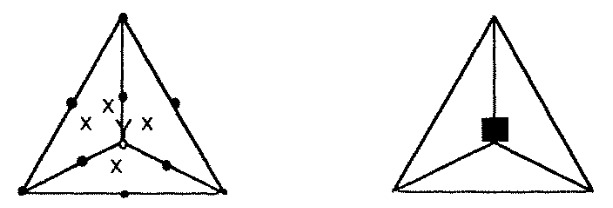
\includegraphics[width=6cm]{images/pair_cr/cr}\\
{\captionfont Taken from \textcite{begt92} (1992).}
\end{center}

The 3D version of this element is presented in \textcite{begt92} (1992). 
In their Table III we find the following node coordinates and basis functions:
\[
\begin{array}{lll}
\text{\# node} & \text{coordinates} & \text{basis function} \\
1  & (0,0,0) & \bN_1(r,s,t)=(1-r-s-t) -\frac12 (\bN_5+\bN_7+\bN_8)-\frac13(\bN_{11}+\bN_{12}+\bN_{13})-\bN_{15}/4 \\ 
2  & (1,0,0) & \bN_2(r,s,t)=r-\frac12(\bN_5+\bN_6+\bN_9)    -\frac13(\bN_{11}+\bN_{12}+\bN_{14}) -\bN_{15}/4 \\
3  & (0,1,0) & \bN_3(r,s,t)=s-\frac12(\bN_6+\bN_7+\bN_{10}) -\frac13(\bN_{11}+\bN_{13}+\bN_{14}) -\bN_{15}/4 \\
4  & (0,0,1) & \bN_4(r,s,t)=t-\frac12(\bN_8+\bN_9+\bN_{10}) -\frac13(\bN_{12}+\bN_{13}+\bN_{14}) -\bN_{15}/4 \\
5  & (\frac12,0,0)             &  \bN_5(r,s,t)=4(1-r-s-t)r-\frac49(\bN_{11}+\bN_{12})-\bN_{15}/4  \\
6  & (\frac12,\frac12,0)       &  \bN_6(r,s,t)=4rs-\frac49(\bN_{11}+\bN_{14})-\bN_{15}/4  \\
7  & (0,\frac12,0)             &  \bN_7(r,s,t)=4(1-r-s-t)s-\frac49(\bN_{11}+\bN_{13})-\bN_{15}/4  \\
8  & (0,0,\frac12)             &  \bN_8(r,s,t)=4(1-r-s-t)t-\frac49(\bN_{12}+\bN_{13})-\bN_{15}/4  \\
9  & (\frac12,0,\frac12)       &  \bN_9(r,s,t)=4rt-\frac49(\bN_{12}+\bN_{14})-\bN_{15}/4  \\
10 & (0,\frac12,\frac12)       &  \bN_{10}(r,s,t)= 4st-\frac49(\bN_{13}+\bN_{14})-\bN_{15}/4 \\
11 & (\frac13,\frac13,0)       &  \bN_{11}(r,s,t)= 27(1-r-s-t)rs-\frac{108}{256}\bN_{15} \\
12 & (\frac13,0,\frac13)       &  \bN_{12}(r,s,t)= 27(1-r-s-t)rt-\frac{108}{256}\bN_{15} \\
13 & (0,\frac13,\frac13)       &  \bN_{13}(r,s,t)= 27(1-r-s-t)st-\frac{108}{256}\bN_{15} \\
14 & (\frac13,\frac13,\frac13) &  \bN_{14}(r,s,t)= 27rst-\frac{108}{256}\bN_{15} \\
15 & (\frac14,\frac14,\frac14) &  \bN_{15}(r,s,t)= 256(1-r-s-t)rst \\
\end{array}
\]

We have
\begin{eqnarray}
\bN_1+\bN_2+\bN_3+\bN_4 
&=& (1-r-s-t) -\frac12 (\bN_5+\bN_7+\bN_8)-\frac13(\bN_{11}+\bN_{12}+\bN_{13})-\bN_{15}/4 \nn\\
&+& r-\frac12(\bN_5+\bN_6+\bN_9)    -\frac13(\bN_{11}+\bN_{12}+\bN_{14}) -\bN_{15}/4 \\
&+& s-\frac12(\bN_6+\bN_7+\bN_{10}) -\frac13(\bN_{11}+\bN_{13}+\bN_{14}) -\bN_{15}/4 \\
&+& t-\frac12(\bN_8+\bN_9+\bN_{10}) -\frac13(\bN_{12}+\bN_{13}+\bN_{14}) -\bN_{15}/4 \\
&=& 1 -\frac12(1+1)\bN_5 -\frac12(1+1)\bN_6 -\frac12(1+1)\bN_7 -\frac12(1+1)\bN_8 -\frac12(1+1)\bN_9 -\frac12(1+1)\bN_{10}    \nn\\
&&  -\frac13(1+1+1)\bN_{11} -\frac13(1+1+1)\bN_{12} -\frac13(1+1+1)\bN_{13} -\frac13(1+1+1)\bN_{14} 
-\frac{1}{4}(1+1+1+1)\bN_{15} \nn\\
&=& 1 -\bN_5 -\bN_6 -\bN_7 -\bN_8 -\bN_{9} -\bN_{10}
      -\bN_{11} -\bN_{12} -\bN_{13} -\bN_{14} -\bN_{15} 
\end{eqnarray}
So in the end
\[
\sum_{i=1}^{15} \bN_i = (\bN_1+\bN_2+\bN_3+\bN_4)  + \sum_{i=5}^{15} \bN_i = 0
\]

\begin{center}
\url{https://defelement.com/elements/conforming-crouzeix-raviart.html}
\end{center}





%------------------------------------------------------------------------------
\subsection{The ${ P}_2^+\times P_{1}$ pair \label{ss:p2pp1}}
\begin{flushright} {\tiny {\color{gray} \tt  pair\_p2pp1.tex}} \end{flushright}
%~~~~~~~~~~~~~~~~~~~~~~~~~~~~~~~~~~~~~~~~~~~~~~~~~~~~~~~~~~~~~~~~~~~~~~~~~~~~~~~~~~~~~~~~~~~~~~~~~~

This element pair is not to be mistaken for the Crouzeix-Raviart. Both share the same $P_2^+$ space
for the velocity but this element has a continuous linear pressure.  
It is mentioned in Table~3.13-1 of \textcite{grsa}: ``LBB stable. Second order. cubic bubble. good element''.
It is also mentioned in \textcite{sofo87} (1987).

Implemented in \stone~120.


%------------------------------------------------------------------------------
\subsection{The ${ P}_2\times (P_1+P_0)$ pair} \label{ss:p2p1p0}
\begin{flushright} {\tiny {\color{gray} \tt pair\_p2p1p0.tex}} \end{flushright}
%~~~~~~~~~~~~~~~~~~~~~~~~~~~~~~~~~~~~~~~~~~~~~~~~~~~~~~~~~~~~~~~~~~~~~~~~~~~~~~~~~~~~~~~~~~~~~~~~~~

This element pair is discussed in 5.3.3 of Elman, Silvester and Wathen: 
\begin{displayquote}
{\color{darkgray}
[Another] possibility is to construct a hybrid pressure approximation by 
combining the continuous linear pressure approximation with the 
discontinuous constant pressure approximation. The resulting mixed method 
is referred to as the $P_2-P_{-1*}$ 
approximation and enjoys the best of both worlds; it has locally 
incompressibility, and yet it does not have its accuracy compromised by
the lower order pressure [of $P_2\times P_0$]. 
Perhaps surprisingly, this element is also uniformly stable.
}
\end{displayquote}

\begin{center}
\includegraphics[width=7cm]{images/pair_p2p1p0/elsw}\\
{\captionfont Taken from \textcite{elsw}.}
\end{center}

In Gresho \& Sani table 3.13-1: 
``LBB stable yes. Better than P2P1, element mass balance.
more work than P2P1. 2 hydrostatic modes. Second order.'' 

\begin{center}
\includegraphics[width=4cm]{images/pair_p2p1p0/grsa2}
\includegraphics[width=12cm]{images/pair_p2p1p0/grsa1}\\
{\captionfont Taken from \textcite{grsa}. Unfortunately they do not 
provide a source for 
its origin, for the LBB-stability proof, or any source at all, actually.}
\end{center}

Looking at the figure above, it is clear that the $P_1$ space is to be understood 
as a continuous pressure space, with an additional constant bubble. 

For the continuous $P_1$ space, we have the following reference element
\begin{center}
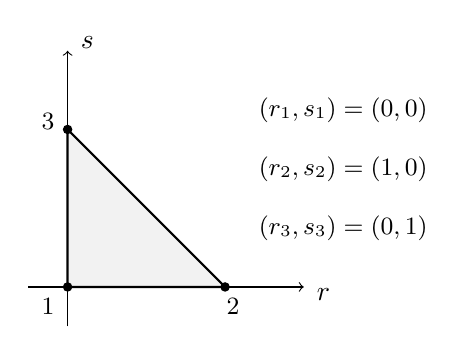
\begin{tikzpicture}
\draw[fill=gray!10,gray!10] (0.5,0.5)--(2.5,0.5)--(0.5,2.5)--cycle;
\draw[thick] (0.5,0.5)--(2.5,0.5)--(0.5,2.5)--cycle;
\draw [->] (0,0.5) -- (3.5,0.5);
\draw [->] (0.5,0) -- (0.5,3.5);
\node[] at (3.75,0.4) {$r$};
\node[] at (0.75,3.6) {$s$};
\draw[black,fill=black] (0.5,0.5)   circle (1.5pt);
\draw[black,fill=black] (2.5,0.5)   circle (1.5pt);
\draw[black,fill=black] (0.5,2.5)   circle (1.5pt);
\node[] at (0.25,0.25) {\small $1$};
\node[] at (2.6,0.25) {\small $2$};
\node[] at (0.25,2.6) {\small $3$};
\node[] at (4,2.75) {\small $(r_1,s_1)=(0,0)$};
\node[] at (4,2) {\small $(r_2,s_2)=(1,0)$};
\node[] at (4,1.25) {\small $(r_3,s_3)=(0,1)$};
\end{tikzpicture}
\end{center}
and the basis functions are simply
\begin{eqnarray}
\bN_1(r,s) &=& 1-r-s \\
\bN_2(r,s) &=& r \\
\bN_3(r,s) &=& s 
\end{eqnarray}
with the interpolation requirement $\bN_i(r_j,s_j)=\delta_{ij}$ fulfilled, 
as well as $\sum_i \bN_i=1$. 

Now, following the figure by Gresho and Sani, I build the reference element for the $P_1+P_0$ space:
\begin{center}
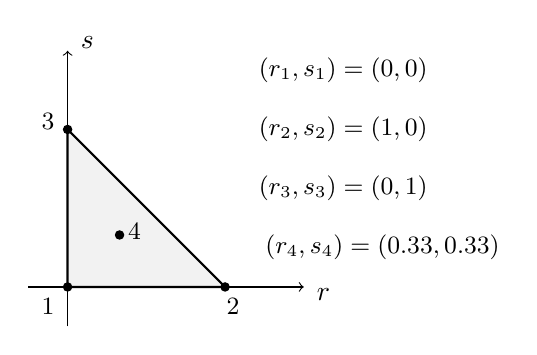
\begin{tikzpicture}
\draw[fill=gray!10,gray!10] (0.5,0.5)--(2.5,0.5)--(0.5,2.5)--cycle;
\draw[thick] (0.5,0.5)--(2.5,0.5)--(0.5,2.5)--cycle;
\draw [->] (0,0.5) -- (3.5,0.5);
\draw [->] (0.5,0) -- (0.5,3.5);
\node[] at (3.75,0.4) {$r$};
\node[] at (0.75,3.6) {$s$};
\draw[black,fill=black] (0.5,0.5)   circle (1.5pt);
\draw[black,fill=black] (2.5,0.5)   circle (1.5pt);
\draw[black,fill=black] (0.5,2.5)   circle (1.5pt);
\draw[black,fill=black] (1.16,1.16) circle (1.5pt);
\node[] at (0.25,0.25) {\small $1$};
\node[] at (2.6,0.25) {\small $2$};
\node[] at (0.25,2.6) {\small $3$};
\node[] at (1.35,1.2) {\small $4$};
\node[] at (4,3.25) {\small $(r_1,s_1)=(0,0)$};
\node[] at (4,2.5)    {\small $(r_2,s_2)=(1,0)$};
\node[] at (4,1.75) {\small $(r_3,s_3)=(0,1)$};
\node[] at (4.5,1) {\small $(r_4,s_4)=(0.33,0.33)$};
\end{tikzpicture}
\end{center}

$P_1+P_0$ means that the pressure inside the element is given by
\[
p^h(r,s) = a \bN_1(r,s)+ b\bN_2(r,s) + c\bN_3(r,s) + d\bN_4(r,s) 
\]
Note that it is then impossible to find $a,b,c,d$ such that the interpolation 
requirement $\bN_i(r_j,s_j)=\delta_{ij}$ is fulfilled.
In other words, the element is not interpolatory, i.e., there is no $\delta_{ij}$ property.% W.B. email

With regards to the 'element mass balance', W.B. states : 
\begin{displayquote}
{\color{darkgray}
the mass conservation requires that the function that is constant 1 
on one cell and zero on all other cells is part of the function space. 
That is indeed true -- it's the $\bN_4$ function. Indeed, that's the purpose of 
the enrichment with the $P_0$ part. It is not necessary that {\it all} shape functions are discontinuous.
}
\end{displayquote}




\textcite{bocg12} (2012) state: 
\begin{displayquote}
{\color{darkgray}
[...] the pressure space $Q_h$ is defined as the sum of two finite 
element spaces, namely $P_k+P_0$ ($k \ge d- 1$) [...] for the enhanced 
Hood–Taylor [...]. However, it can be easily observed that the sum is not direct, 
since globally constant functions can be represented exactly by means of piecewise 
$P_0$ or continuous $P_k$ ($k \ge 1$) elements.
Concerning the implementation of the method, we avoid the computation of the basis
functions of such a finite element by testing the discrete problem (2.3) 
with the basis 
functions of the two subspaces separately. By the above discussion it 
turns out that the resulting
matrix is rank-deficient, with kernel of dimension 1.
}
\end{displayquote}

The element pair is also discussed in \textcite{chen14} (2014).



%------------------------------------------------------------------------------
\subsection{The ${ P}_3\times P_2$ pair} \label{ss:p3p2}
\index{general}{$P_3\times P_2 element$}
\begin{flushright} {\tiny {\color{gray} \tt pair\_p3p2.tex}} \end{flushright}
%~~~~~~~~~~~~~~~~~~~~~~~~~~~~~~~~~~~~~~~~~~~~~~~~~~~~~~~~~~~~~~~~~~~~~~~~~~~~~~~~~~~~~~~~~~~~~~~~~~

${\bm P}_3\times P_2$ mentioned in \textcite{sten90}.
The $P_3$ basis functions are presented in Section~\ref{basis:p3} and the $P_2$ basis
functions in Section~\ref{basis:p2}.
See \stone~120.


%------------------------------------------------------------------------------
\subsection{The $P_4\times P_3$ pair} \label{ss:p4p3}
It is implemented in \stone~120.
The $P_4$ and $P_3$ spaces are defined in Sections~\ref{basis:p4} and \ref{basis:p3} respectively.



%------------------------------------------------------------------------------
\subsection{The Raviart-Thomas family} \label{ss:raviart_thomas}
\begin{flushright} {\tiny {\color{gray} \tt pair\_raviart\_thomas.tex}} \end{flushright}
%~~~~~~~~~~~~~~~~~~~~~~~~~~~~~~~~~~~~~~~~~~~~~~~~~~~~~~~~~~~~~~~~~~~~~~~~~~~~~~~~~~~~~~~~~~~~~~~~~~

- Raviart Thomas 0 RT0 \cite{rath77} ? mentioned/defined/drawn in 4.2.2 of 
Kanschat book. Also exist for quads see 4.2.37 
\textcite{hald03}: ``$P_1^\perp \times P_0$ symbol denotes an element with 
normal velocity nodes in the middle of each edge of the
triangulation [...]. This element, also called low order Raviart–Thomas element 
(Raviart and Thomas, 1977), is based on flux conservation on elements edges and 
the resulting scheme is very close to a finite volume scheme.''

Mentioned in \textcite{john16}, appendix B.3, example B.45: ``the normal component of v 
on each face is a constant. The normal component of functions from RT0 is
continuous across faces of the mesh cells.''

Check \textcite{brfo}

Mentioned in \textcite{chen93a} (1993).

\url{https://defelement.com/elements/raviart-thomas.html}


\url{
https://en.wikipedia.org/wiki/Raviart-Thomas_basis_functions
}

\url{
https://people.tamu.edu/~guermond//M661_FALL_2015/chap7.pdf
}

\url{
https://scicomp.stackexchange.com/questions/20245/raviart-thomas-elements-on-reference-square
}





%------------------------------------------------------------------------------
\subsection{The Bernardi-Raugel pair} \label{ss:bernardi_raugel}
\begin{flushright} {\tiny {\color{gray} \tt pair\_bernardi\_raugel.tex}} \end{flushright}
%~~~~~~~~~~~~~~~~~~~~~~~~~~~~~~~~~~~~~~~~~~~~~~~~~~~~~~~~~~~~~~~~~~~~~~~~~~~~~~~~~~~~~~~~~~~~~~~~~~

In \textcite{cakp15} (2015) we find: ``The BR-FEM after Bernardi and Raugel \cite{bera85} 
is a modification of the $P_2\times P_0$ FEM. It is sometimes also called reduced $P_2\times P_0$ FEM''.
They also state that this element also exists in 3D.

\begin{center}
\includegraphics[width=5cm]{images/pair_bernardi_raugel/cakp15}
\end{center}

It is also mentioned in \textcite{bobf13} although it seems it is there called the SMALL element (p474).

In Lederer: "Consider the case d = 2. [...] we only need to control 
the normal velocity at the edge, i.e. adding the
edge bubble for both components of the velocity seems to be sub optimal (with respect to
computational costs and the expected approximation properties). The idea now is to only
add the normal edge bubble."

According to \textcite{jolm17} (2017) (example 6.3), `` the velocity space in the Bernardi-Raugel
element consists of $P_1$ functions which are enriched with edge bubble functions''.
The authors also speak of 'reconstructing the test functions' and state: 
``the results of the method with reconstruction are generally more accurate.
In summary, the use of an appropriately reconstructed test function in the Bernardi–
Raugel pair of spaces led to a clear improvement of the accuracy of the computed
results compared with the standard method.''

In \cite{befh21} the authors use the so-called Extended Bernardi-Raugel (EBR) element
which they call $(P_1 + B_3^F)^3 - P_0$ ``which is a cheap and stable pairing with few degrees of
freedom (DOFs) per cell''.

\url{https://defelement.com/elements/bernardi-raugel.html}




\newpage
%------------------------------------------------------------------------------
\subsection{The Scott-Vogelius pair} \label{ss:scott_vogelius}
\index{general}{Scott-Vogelius pair}
\begin{flushright} {\tiny {\color{gray} \tt pair\_scott\_vogelius.tex}} \end{flushright}
%~~~~~~~~~~~~~~~~~~~~~~~~~~~~~~~~~~~~~~~~~~~~~~~~~~~~~~~~~~~~~~~~~~~~~~~~~~~~~~~~~~~~~~~~~~~~~~~~~~

It originates in \fullcite{scvo85} (1985). 

 
In Remark 9 (p.29) of \textcite{aubb17} (2017) we find: 
\begin{displayquote}
{\color{darkgray}
We also remark that the discontinuous
pressure version of the Hood–Taylor element typically
results in an unstable method. However, stability can be
recovered by imposing certain restrictions on the mesh for
$k \ge 3$ (see \cite{voge83}; \cite{scvo85}), or
by taking advantage of suitable stabilization procedures for
$k\ge 1$ (see Mansfield, 1982; Boffi, 1995).
}
\end{displayquote}

In \textcite{fams21} (2021) we find:
\begin{displayquote}
{\color{darkgray}
The Scott-Vogelius element is given by choosing continuous piecewise 
polynomials of degree $k$ for the velocity and discontinuous piecewise 
polynomials of degree $k-1$ for the pressure. While this clearly
implies that $\nabla\cdot V_h \in Q_h$, inf-sup stability of the 
Scott–Vogelius element is more delicate, and is a topic of ongoing research. 
In two dimensions, Scott \& Vogelius proved \cite{scvo85} that the element is inf-sup
stable for $k\ge 4$ if the mesh does not have nearly singular vertices. 
In three dimensions, it was proven more recently in \cite{zhan11b} 
that the element is stable for $k\ge 6$ on uniform meshes. The stability on general
tetrahedral meshes continues to be an open question.

On barycentrically refined meshes, however, the pair is known to 
be stable for polynomial order
$k = d$, see [48, Section 4.6] for the 2D case and 
\cite{zhan05} for the 3D case. If one is willing to 
consider the more complicated Powell–Sabin split, the order 
can be reduced further to $k=d-1$ \cite{zhan08,zhan11a}. The two
refinement patterns are shown for the two dimensional case 
in Figure 1 [see below]. In this work we will consider
the case of $k \ge d$ on barycentrically refined meshes, but 
the arguments apply mutatis mutandis to the Powell–Sabin split.
}
\end{displayquote}

\begin{center}
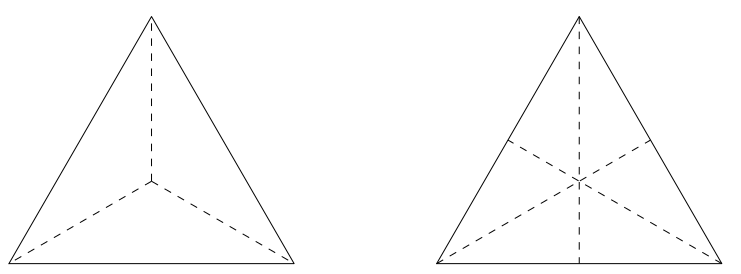
\includegraphics[width=9cm]{images/pair_scott_vogelius/scottvogelius_split}\\
{\captionfont 
Barycentrically refined triangle (also known as Alfeld split) on the left,
and Powell–Sabin split on the right.\\ Taken from \textcite{fams21} (2021).}
\end{center}

\index{general}{Powell-Sabin}

\textcite{cael11} (2011) state:
\begin{displayquote}
{\color{darkgray}
The SV element pair is not yet very well known,
and so we now give a brief description of it. In essence, the SV pair is the same as
the Taylor-Hood pair except that the pressure space is discontinuous and either
(i) for $k \ge d$, the mesh is a barycenter refinement of a regular mesh, or
(ii) for $k = 2, d = 3$, the mesh is formed from a barycenter refined mesh by
connecting the barycenter nodes (i.e., a Powell–Sabin tetrahedralization).
In short, polynomials of degree $k$ and $k-1$ are used to approximate the velocity
and pressure spaces, respectively, and the mesh ${\cal T}_h$ that is used must be derived from
a regular triangulation (tetrahedralization) of $\Omega$, where each element is refined as
stated above. With these mesh constructions, it was proved by Zhang in [42, 44] that
the SV elements are LBB stable, and, consequently, also have optimal approximation
properties. It is well known that the TH pair is LBB stable and admits optimal
approximation properties for these cases as well [9]. We will restrict our definition of
SV elements to these cases where they are LBB stable.
}
\end{displayquote}

On page 112 of \textcite{john16} we read:
\begin{displayquote}
{\color{darkgray}
The Scott–Vogelius finite element considers still $P_k/P^{disc}_{k-1}$, $k \ge d$, 
but on special meshes, which allow to show the satisfaction of the 
discrete inf-sup condition.
[...]
This pair of finite element spaces $P_k/P^{disc}_{k-1}$
are weakly divergence-free, which is a desirable property.
[...]
The fulfillment of the discrete inf-sup condition 
was proved already in \textcite{scvo85} (1985) in the two-dimensional 
case for $k\ge 4$ if there is no so-called singular vertex in the mesh.
An internal vertex is said to be singular if edges which meet at the vertex fall onto
two straight lines.

The basic idea to overcome this problem consists in using meshes 
without singular vertices. To this end, so-called barycentric-refined 
grids are constructed. Starting from any admissible triangular mesh, 
new edges are introduced by connecting all
vertices of a mesh cell with the barycenter of this mesh cell. 
This step creates smaller triangles.
On barycentric-refined meshes, the $P_k/P^{disc}_{k-1}$, $k=2,3$ 
pair of finite element spaces was shown to satisfy the discrete inf-sup
condition in Qin's phd thesis (1994). [...]

The use of the $P_2/P^{disc}_{1}$ pair of finite element spaces 
on barycentric-refined meshes can be found occasionally in the literature,
in particular to demonstrate the advantages of using pairs of finite element 
spaces which provide weakly divergence-free velocity solutions, 
e.g. see \textcite{john15} and refs therein.

}
\end{displayquote}


\begin{center}
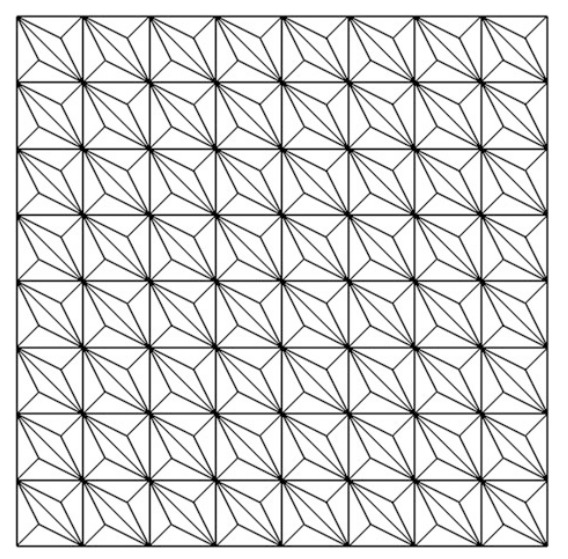
\includegraphics[width=6cm]{images/pair_scott_vogelius/john16}\\
{\captionfont Barycentric-refined simplicial grid on the unit square}
\end{center}

I hereafter present my own internal numbering for the mesh above (used in \stone~120 for example).
The quadrilateral has been cut once along a diagonal, and then an Alfeld split is used, thereby 
dividing the square in 6 triangles:

\begin{flushright} {\tiny {\color{gray} (tikz\_sv.tex)}} \end{flushright}
%~~~~~~~~~~~~~~~~~~~~~~~~~~~~~~~~~~~~~~~~~~~~~~~~~~~~~~~~~~~~~~~~~~~~~~~~~~~~~~~~~~~~~~~~~~~~~~~~~~


\begin{center} 
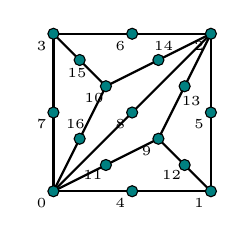
\begin{tikzpicture} 

%\draw[fill=gray!23,gray!23](0,0) rectangle (2.5,2.5);
%\draw[step=0.5cm,gray,very thin] (0,0) grid (2.5,2.5); %background grid

%ielx=1,iely=1,low
\draw[thick] (0,0)--(1.33333,0.66667);
\draw[thick] (2,0)--(1.33333,0.66667);
\draw[thick] (2,2)--(1.33333,0.66667);
%ielx=1,iely=1,high
\draw[thick] (0,0)--(0.666667,1.3333);
\draw[thick] (0,2)--(0.666667,1.3333);
\draw[thick] (2,2)--(0.666667,1.3333);

\draw[thick] (0,0) -- (2,0) -- (2,2) -- (0,2) -- cycle; 
\draw[thick] (0,0) -- (2,2) ; %diag


%\draw[thick] (6,0) -- (4,2) -- (6,4) ; 
\draw[black,fill=teal] ( 0.000000 , 0.000000)     circle (2pt); 
\node[] at ( -0.150000, -0.150000 ) {\tiny 0 }; 
\draw[black,fill=teal] ( 2.000000 , 0.000000)     circle (2pt); 
\node[] at ( 1.850000, -0.150000 ) {\tiny 1 }; 
\draw[black,fill=teal] ( 2.000000 , 2.000000)     circle (2pt); 
\node[] at ( 1.850000, 1.850000 ) {\tiny 2 }; 
\draw[black,fill=teal] ( 0.000000 , 2.000000)     circle (2pt); 
\node[] at ( -0.150000, 1.850000 ) {\tiny 3 }; 
\draw[black,fill=teal] ( 1.000000 , 0.000000)     circle (2pt); 
\node[] at ( 0.850000, -0.150000 ) {\tiny 4 }; 
\draw[black,fill=teal] ( 2.000000 , 1.000000)     circle (2pt); 
\node[] at ( 1.850000, 0.850000 ) {\tiny 5 }; 
\draw[black,fill=teal] ( 1.000000 , 2.000000)     circle (2pt); 
\node[] at ( 0.850000, 1.850000 ) {\tiny 6 }; 
\draw[black,fill=teal] ( 0.000000 , 1.000000)     circle (2pt); 
\node[] at ( -0.150000, 0.850000 ) {\tiny 7 }; 
\draw[black,fill=teal] ( 1.000000 , 1.000000)     circle (2pt); 
\node[] at ( 0.850000, 0.850000 ) {\tiny 8 }; 
\draw[black,fill=teal] ( 1.333333 , 0.666667)     circle (2pt); 
\node[] at ( 1.183333, 0.516667 ) {\tiny 9 }; 
\draw[black,fill=teal] ( 0.666667 , 1.333333)     circle (2pt); 
\node[] at ( 0.516667, 1.183333 ) {\tiny 10 }; 
\draw[black,fill=teal] ( 0.666667 , 0.3333)     circle (2pt); 
\node[] at ( 0.5, 0.2 ) {\tiny 11 }; 
\draw[black,fill=teal] ( 1.6667 , 0.3333)     circle (2pt); 
\node[] at ( 1.5, 0.2 ) {\tiny 12 }; 
\draw[black,fill=teal] ( 1.6667 , 1.3333)     circle (2pt); 
\node[] at ( 1.75, 1.15 ) {\tiny 13 }; 
\draw[black,fill=teal] ( 0.3333,0.666667)     circle (2pt); 
\node[] at ( 1.4,1.85 ) {\tiny 14}; 
\draw[black,fill=teal] ( 0.3333, 1.6667)     circle (2pt); 
\node[] at ( 0.3,1.5 ) {\tiny 15 }; 
\draw[black,fill=teal] ( 1.3333, 1.6667)     circle (2pt); 
\node[] at ( 0.28,0.85 ) {\tiny 16 }; 


\end{tikzpicture} 
%\end{center} 


%\begin{center} 
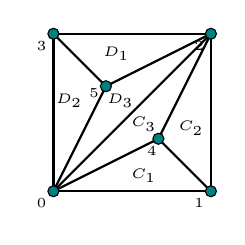
\begin{tikzpicture} 

%\draw[fill=gray!23,gray!23](0,0) rectangle (2.5,2.5);
%\draw[step=0.5cm,gray,very thin] (0,0) grid (2.5,2.5); %background grid

%ielx=1,iely=1,low
\draw[thick] (0,0)--(1.33333,0.66667);
\draw[thick] (2,0)--(1.33333,0.66667);
\draw[thick] (2,2)--(1.33333,0.66667);
%ielx=1,iely=1,high
\draw[thick] (0,0)--(0.666667,1.3333);
\draw[thick] (0,2)--(0.666667,1.3333);
\draw[thick] (2,2)--(0.666667,1.3333);

\draw[thick] (0,0) -- (2,0) -- (2,2) -- (0,2) -- cycle; 
\draw[thick] (0,0) -- (2,2) ; %diag

%\draw[thick] (6,0) -- (4,2) -- (6,4) ; 
\draw[black,fill=teal] ( 0.000000 , 0.000000)     circle (2pt); 
\node[] at ( -0.150000, -0.150000 ) {\tiny 0 }; 
\draw[black,fill=teal] ( 2.000000 , 0.000000)     circle (2pt); 
\node[] at ( 1.850000, -0.150000 ) {\tiny 1 }; 
\draw[black,fill=teal] ( 0.000000 , 2.000000)     circle (2pt); 
\node[] at ( -0.150000, 1.850000 ) {\tiny 3 }; 
\draw[black,fill=teal] ( 2.000000 , 2.000000)     circle (2pt); 
\node[] at ( 1.850000, 1.850000 ) {\tiny 2 }; 
\draw[black,fill=teal] ( 1.333333 , 0.666667)     circle (2pt); 
\node[] at ( 1.25, 0.516667 ) {\tiny 4 }; 
\draw[black,fill=teal] ( 0.666667 , 1.333333)     circle (2pt); 
\node[] at ( 0.516667, 1.25 ) {\tiny 5 }; 

\node[] at ( 1.15,0.2 ) {\tiny $C_1$ }; 
\node[] at ( 1.75,0.8 ) {\tiny $C_2$ }; 
\node[] at ( 1.15,0.85 ) {\tiny $C_3$ }; 

\node[] at ( 0.8,1.75 ) {\tiny $D_1$ }; 
\node[] at ( 0.2,1.15 ) {\tiny $D_2$ }; 
\node[] at ( 0.85,1.15 ) {\tiny $D_3$ }; 

\end{tikzpicture} 
\end{center} 



See also \textcite{jolm17} (2017) in which the $P_2\times P_1$, Scott-Vogelius ($P_2\times P_{-1}$), 
Bernardi-Raugel, and $P_2^+\times P_{-1}$ elements 
are compared for a thermo-mechanically driven convection problem in a triangle (see \stone~51, 
although I use the $P_1^+\times P_1$ element in this stone).


\begin{center}
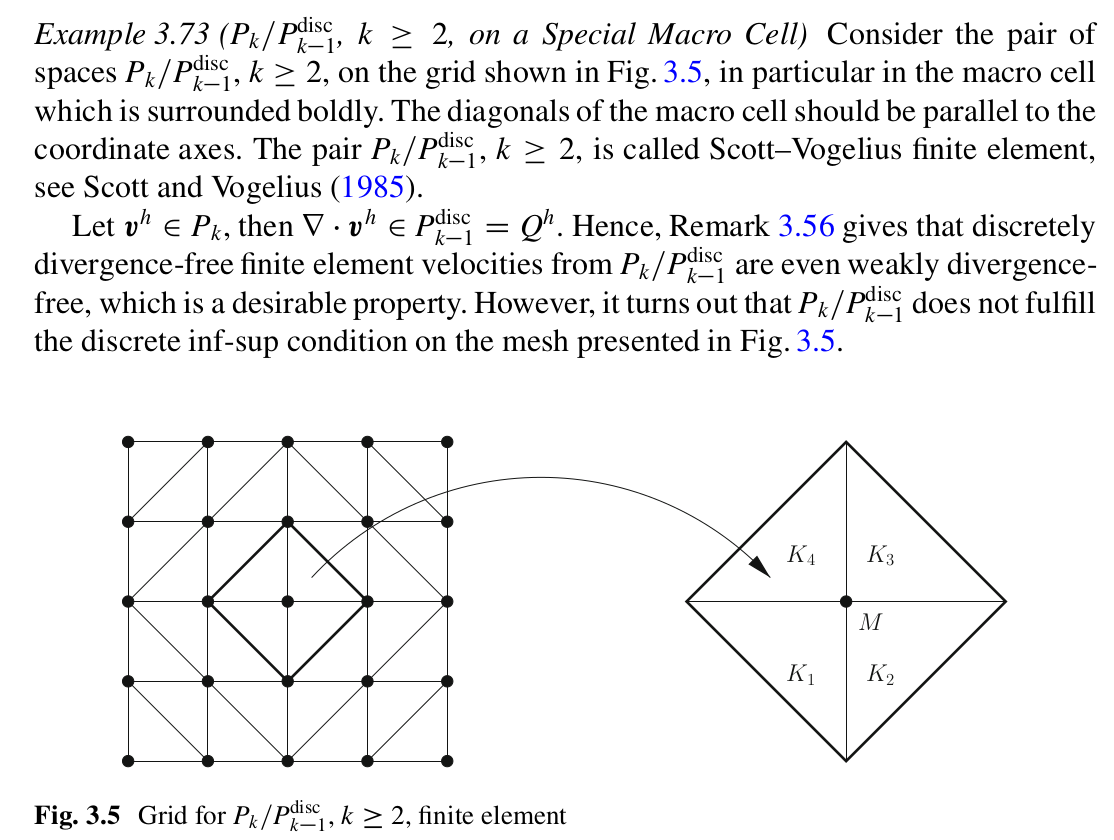
\includegraphics[width=10cm]{images/pair_scott_vogelius/john_scott_vogelius}\\
\captionfont{Taken from John \cite[p70]{john16}.} 
\end{center}


In \textcite{befh21} (2021) this element is used in its 
$(P_3)^2-P_2^{\text{disc}}$ form.

Note that some have proposed to use an incenter-based refinement instead of
a barycenter refinement since it lead to less pronounced aspect ratios\footnote{
The Scott-Vogelius Method for Stokes Problem on Anisotropic Meshes, K Kean, M Neilan, M Schneier,
\url{https://doi.org/10.48550/arXiv.2109.14780}}.
In geometry, the incenter of a triangle is a triangle center, a point defined for 
any triangle in a way that is independent of the triangle's placement or scale. 
The incenter may be equivalently defined as the point where the internal angle bisectors 
of the triangle cross or as the point equidistant from the triangle's sides.

Given the coordinates of the three vertices of a triangle ABC,
the coordinates of the incenter O are
\[
x_O=\frac{ax_A+bx_B+cx_C}{a+b+c}
\qquad
y_O=\frac{ay_A+by_B+cy_C}{a+b+c}
\] 
where $a$, $b$ and $c$ are the side lengths opposite vertex A, B and C.

 
Note that \textcite{zhan24} (2024) proposes a solution to the unstable issue: 
\begin{displayquote}
{\color{darkgray}
We show that the discrete velocity solution converges at
the optimal order when solving the steady state Stokes
equations by the ${\bm P}_k\times P_{-(k-1)}$ mixed finite element method for
$k \ge 4$ on 2D triangular grids or $k \ge 6$ on tetrahedral grids,
even in the case the inf-sup condition fails. By a simple
$L_2$-projection of the discrete $P_{k-1}$ pressure to the space of
continuous $P_{k-1}$ polynomials, we show this post-processed
pressure solution also converges at the optimal order. Both
2D and 3D numerical tests are presented, verifying the
theory.
}
\end{displayquote}

Rather interestingly, we find in \textcite{tesk12} (2012) a penalty-approach:
\begin{displayquote}
{\color{darkgray}
Other solutions to deal with the LBB condition include the Uzawa iteration method and penalty
methods. A combination of these two approaches results in the iterated penalty method presented in
Scott and Vogelius (1985). Let $r\in\R$ and $\rho\in\R^+$ be prescribed parameters. 
We wish to find $u^n\in V_h$ such that 
\[
a(u^n,v) + r(\nabla\cdot u^n,\nabla\cdot v) = (f,v) - (\nabla \cdot v, \nabla\cdot w^n)
\qquad \forall \; v\in V_h,
\]
where $w^{n+1}=w^n+\rho u^n$.
The pressure may be recovered from the auxiliary field $w$ via $p=\nabla\cdot w -C$, 
where $C$ is an arbitrary constant (since the pressure field is only determined up 
to an arbitrary constant). When computing the error in $p$, we subtract the average 
of $\nabla\cdot w$ to account for $C$. The algorithm initially assumes
$w^0=0$, and then solves [the equation above] and updates $w$. 
The process is repeated until $\| u^{n+1}-u^n\|<\epsilon$, 
where $\epsilon$ is a prescribed tolerance. This method involves only one function space, but
it requires a higher-order continuous element $(q\ge 4)$ and it solves the divergence-free criterion
exactly. The iteration count and accuracy are dependent upon the penalty parameters $\rho$ and $r$. 
The implementation of this formulation is presented in [the following figure]:
\begin{center}
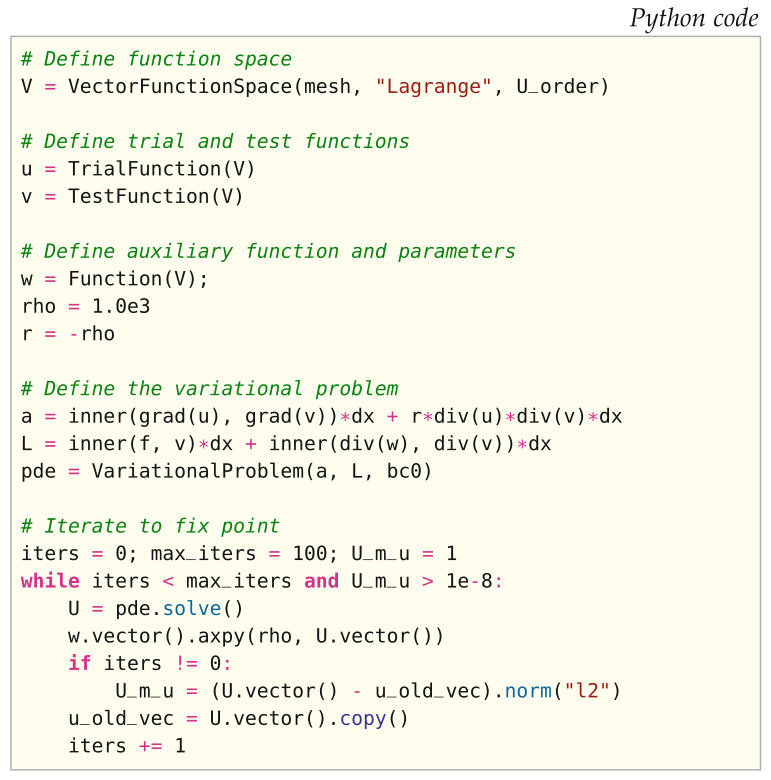
\includegraphics[width=6cm]{images/pair_scott_vogelius/tesk12}
\end{center}

}
\end{displayquote}



\begin{center}
\url{https://defelement.com/elements/scott-vogelius.html}
\end{center}




%------------------------------------------------------------------------------
\subsection{The BDM (Brezzi-Douglas-Marini) pair} \label{ss:bdm}
\index{general}{BDM element}
\begin{flushright} {\tiny {\color{gray} \tt  pair\_bdm.tex}} \end{flushright}
%~~~~~~~~~~~~~~~~~~~~~~~~~~~~~~~~~~~~~~~~~~~~~~~~~~~~~~~~~~~~~~~~~~~~~~~~~~~~~~~~~~~~~~~~~~~~~~~~~~

This element is mentioned in Kanschat book \cite{kanschat}, section 4.2.14. 
It also exists for quads see section 4.2.39 in the same book.
It is mentioned in \textcite{chen93a} (1993), also check the book by \textcite{brfo}.
It is well described in \textcite{kanschat17}.
There is an entire chapter (14) of \textcite{ergu21_72} dedicated to H(div) and 
section 14.5.1 to BDM elements. 
Check section 4.1.1 of \cite{aubb17} for triangles and quads.

\begin{center}
\url{https://defelement.com/elements/brezzi-douglas-marini.html}
\end{center}

\begin{itemize}
%++++++++++++++++++++++++++++++++++++++++++++++
\item In \textcite{lomw12} we read:

The Brezzi-Douglas-Marini element was introduced by Brezzi, Douglas and Marini in two dimensions 
(for triangles) in \textcite{brdm85} (1985). The element can be viewed as an alternative to the
Raviart-Thomas element using a complete polynomial space. It was later extended to three 
dimensions (tetrahedra, prisms and cubes) in \textcite{nede86} (1986) 
and \textcite{brdd87} (1987). The definition given
here is based on that of \textcite{nede86} (1986).

The Brezzi-Douglas-Marini element was introduced for mixed formulations of second-order elliptic 
equations. However, it is also useful for weakly symmetric discretizations of the elastic stress
tensor; see Farhloul and Fortin (1997); Arnold et al. (2007).

\begin{center}
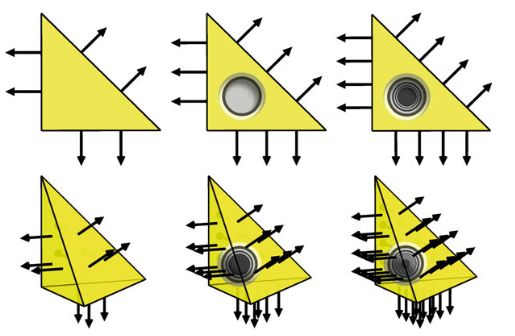
\includegraphics[width=8cm]{images/pair_bdm/bdm_lomw12}\\
{\captionfont Taken from \cite{lomw12}. }
\end{center}

The dimension of $BDM_q$ is $(q+1)(q+2)$ for a triangle and $\frac12(q+1)(q+2)(q+3)$
for a tetrahedron.

Check book for definition.

A slight modification of the Brezzi-Douglas-Marini element constrains the element space ${\cal V}$ by
only allowing normal components on the boundary of polynomial degree $q-1$ (rather than the full
polynomial degree $q$). Such an element was suggested on rectangles by \textcite{brdf87} (1987), and the
triangular analogue was given in \textcite{brfo}. In similar spirit, elements with differing
degrees on the boundary suitable for varying the polynomial degree between triangles were derived
in \textcite{brdm85b} (1985).

%++++++++++++++++++++++++++++++++++++++++++++++
\item On the defelement website\footnote{\url{https://defelement.org/elements/brezzi-douglas-marini.html}}
we find a lot of information. Note that the mapping is set to 'contravariant Piola'. 
\todo[inline]{I still need to understand and write about this!}
It belongs to the categories 'Vector-valued elements', and 'H(div) conforming elements'

\begin{center}
% -------------------------------------------------------
% This plot is from DefElement (https://defelement.org)
% and is available under a Creative Commons Attribution
% 4.0 International (CC BY 4.0) license:
% https://creativecommons.org/licenses/by/4.0/
% -------------------------------------------------------
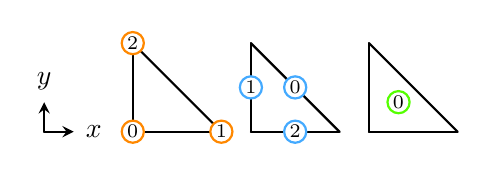
\begin{tikzpicture}[x=1cm,y=1cm]
\definecolor{customcolor0}{HTML}{000000}
\definecolor{customcolor1}{HTML}{44AAFF}
\definecolor{customcolor2}{HTML}{AAAAAA}
\definecolor{customcolor3}{HTML}{DD2299}
\definecolor{customcolor4}{HTML}{FFFFFF}
\definecolor{customcolor5}{HTML}{FF8800}
\definecolor{customcolor6}{HTML}{55FF00}
\draw[-stealth,customcolor0,line width=0.8pt,line cap=round] (25.0,25.0) -- (25.375,25.0);
\draw[-stealth,customcolor0,line width=0.8pt,line cap=round] (25.0,25.0) -- (25.0,25.375);
\node[customcolor0,anchor=west] at (25.405,25.0) {$x$};\node[customcolor0,anchor=south] at (25.0,25.405) {$y$};\draw[customcolor0,line width=0.8pt,line cap=round] (27.25,25.0) -- (26.125,26.125);
\draw[customcolor0,line width=0.8pt,line cap=round] (26.125,25.0) -- (26.125,26.125);
\draw[customcolor0,line width=0.8pt,line cap=round] (26.125,25.0) -- (27.25,25.0);
\draw[customcolor5,line width=0.8pt,fill=customcolor4] (26.125,25.0) circle (4.0pt);
\node[customcolor0,anchor=center] at (26.125,25.0) {\scriptsize 0};\draw[customcolor5,line width=0.8pt,fill=customcolor4] (27.25,25.0) circle (4.0pt);
\node[customcolor0,anchor=center] at (27.25,25.0) {\scriptsize 1};\draw[customcolor5,line width=0.8pt,fill=customcolor4] (26.125,26.125) circle (4.0pt);
\node[customcolor0,anchor=center] at (26.125,26.125) {\scriptsize 2};\draw[customcolor0,line width=0.8pt,line cap=round] (28.75,25.0) -- (27.625,26.125);
\draw[customcolor1,line width=0.8pt,fill=customcolor4] (28.1875,25.5625) circle (4.0pt);
\node[customcolor0,anchor=center] at (28.1875,25.5625) {\scriptsize 0};\draw[customcolor0,line width=0.8pt,line cap=round] (27.625,25.0) -- (27.625,26.125);
\draw[customcolor1,line width=0.8pt,fill=customcolor4] (27.625,25.5625) circle (4.0pt);
\node[customcolor0,anchor=center] at (27.625,25.5625) {\scriptsize 1};\draw[customcolor0,line width=0.8pt,line cap=round] (27.625,25.0) -- (28.75,25.0);
\draw[customcolor1,line width=0.8pt,fill=customcolor4] (28.1875,25.0) circle (4.0pt);
\node[customcolor0,anchor=center] at (28.1875,25.0) {\scriptsize 2};\draw[customcolor6,line width=0.8pt,fill=customcolor4] (29.5,25.375) circle (4.0pt);
\node[customcolor0,anchor=center] at (29.5,25.375) {\scriptsize 0};\draw[customcolor0,line width=0.8pt,line cap=round] (30.25,25.0) -- (29.125,26.125);
\draw[customcolor0,line width=0.8pt,line cap=round] (29.125,25.0) -- (29.125,26.125);
\draw[customcolor0,line width=0.8pt,line cap=round] (29.125,25.0) -- (30.25,25.0);
\end{tikzpicture}
\\
{\captionfont Taken from DefElement \url{https://defelement.org/img/ref-triangle.html}. I have altered 
the font size. Orange: nodes; Blue: edges.}
\end{center}


I reproduce below the figures and basis functions pertaining to the Degree 1 triangle, 
but the site also shows Degree 2 triangle, Degree 1 \& 2 tetrahedron, and so-called 
Lagrange variants.

\begin{center}
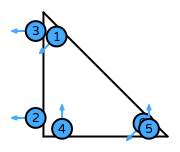
\includegraphics[width=3cm]{images/pair_bdm/element-Brezzi-Douglas-Marini-variant-equispaced-triangle-1-dofs}
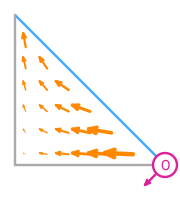
\includegraphics[width=3cm]{images/pair_bdm/element-Brezzi-Douglas-Marini-variant-equispaced-triangle-1-0}
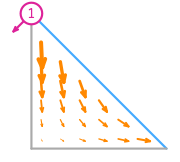
\includegraphics[width=3cm]{images/pair_bdm/element-Brezzi-Douglas-Marini-variant-equispaced-triangle-1-1}
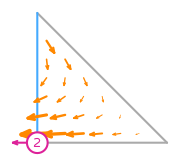
\includegraphics[width=3cm]{images/pair_bdm/element-Brezzi-Douglas-Marini-variant-equispaced-triangle-1-2}\\
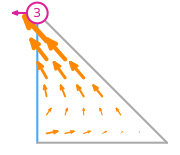
\includegraphics[width=3cm]{images/pair_bdm/element-Brezzi-Douglas-Marini-variant-equispaced-triangle-1-3}
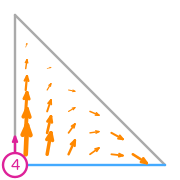
\includegraphics[width=3cm]{images/pair_bdm/element-Brezzi-Douglas-Marini-variant-equispaced-triangle-1-4}
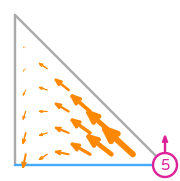
\includegraphics[width=3cm]{images/pair_bdm/element-Brezzi-Douglas-Marini-variant-equispaced-triangle-1-5}\\
{\captionfont Pink: degrees of freedom.}
\end{center}


${\cal V}$ is spanned by 
\[
\left(\begin{array}{c}
1 \\ 0
\end{array}\right),
\left(\begin{array}{c}
0 \\ 1
\end{array}\right),
\left(\begin{array}{c}
x \\ 0
\end{array}\right),
\left(\begin{array}{c}
0 \\ x
\end{array}\right),
\left(\begin{array}{c}
y \\ 0
\end{array}\right),
\left(\begin{array}{c}
0 \\ y
\end{array}\right)
\]
with 
\begin{itemize}
\item DOF \#0 is associated with edge 0 of the reference element with $\vec{\bN}_0$ basis function.
\item DOF \#1 is associated with edge 0 of the reference element with $\vec{\bN}_1$ basis function.
\item DOF \#2 is associated with edge 1 of the reference element with $\vec{\bN}_2$ basis function.
\item DOF \#3 is associated with edge 1 of the reference element with $\vec{\bN}_3$ basis function.
\item DOF \#4 is associated with edge 2 of the reference element with $\vec{\bN}_4$ basis function.
\item DOF \#5 is associated with edge 2 of the reference element with $\vec{\bN}_5$ basis function.
\end{itemize}
and
\begin{eqnarray}
\vec{\bN}_0 &=&  \left(\begin{array}{c} -4x \\ 2y        \end{array}\right) \nn\\  
\vec{\bN}_1 &=&  \left(\begin{array}{c} 2x \\ -4y        \end{array}\right) \nn\\  
\vec{\bN}_2 &=&  \left(\begin{array}{c} 4x+6y-4 \\ -2y   \end{array}\right) \nn\\  
\vec{\bN}_3 &=&  \left(\begin{array}{c} -2x-6y+2 \\ 4y   \end{array}\right) \nn\\  
\vec{\bN}_4 &=&  \left(\begin{array}{c} 2x \\ -6x-4y+4   \end{array}\right) \nn\\  
\vec{\bN}_5 &=&  \left(\begin{array}{c} -4x \\ 6x +2y -2 \end{array}\right) \nn
\end{eqnarray}

 

\item In \cite{brdf87} we read:
\begin{displayquote}
The object of this paper is to present families of rectangular mixed finite
éléments that are derived from the elements of \cite{brdm85} 
in two space variables and of \cite{brdd87} in three space variables.
\end{displayquote}














\end{itemize}



%------------------------------------------------------------------------------
\subsection{The Divergence-free nonconforming ${ P}_1^{NC}\times P_0$ pair} \label{ss:p1ncp0}
\begin{flushright} {\tiny {\color{gray} \tt pair\_p1ncp0.tex}} \end{flushright}
%~~~~~~~~~~~~~~~~~~~~~~~~~~~~~~~~~~~~~~~~~~~~~~~~~~~~~~~~~~~~~~~~~~~~~~~~~~~~~~~~~~~~~~~~~~~~~~~~~~

It belongs to the Crouzeix-Raviart family. 
The midside nodes are used as degrees of freedom for the velocities.
It is mentioned in Section~6.3 of \textcite{bobf08} (2008): 
\begin{displayquote}
{\color{darkgray}
[...]
It is exactly divergence free. Another important feature of this
element is that it can be seen as a "mass conservation" scheme. The present element
has been generalized to second order in \textcite{foso83} (1983).
It must also be said that coerciveness may be a problem for the $P_1^{NC} \times P_0$ 
element, as it does not satisfy the discrete version of Korn's inequality. 
This issue has been deeply investigated and clearly illustrated in \textcite{arno93} (1993).}
\end{displayquote}

\input{tikz/tikz_p1ncp0}

At page 170 of \cite{braess} it is stated that {\color{darkgray} ``an analogous quadrilateral element was 
developed and studied by \textcite{ratu92} (1992)''} (see Section~\ref{ss:RTq1p0}).

In \textcite{bobf13} we find: 
\begin{displayquote}
{\color{darkgray}
We consider the classical (almost\footnote{What does that mean?!}) 
stable nonconforming triangular 
element introduced in \textcite{crra73}, in which mid-side nodes are used as degrees of 
freedom for the velocities. This generates
a piecewise linear nonconforming approximation; pressures are taken constant on
each element. It is also possible to build a three-dimensional
version of this element, using mid-face nodes as degrees of freedom.
\\
..
\\
It must also be recalled that coercivity is a problem for the $P_1^{NC}\times P_0$ 
element. The trouble is that the bilinear form (8.2.1) is not coercive on the 
nonconforming space $V_h$ and we do not have the discrete version of Korn's inequality.}
\end{displayquote}


It is also mentioned in \textcite{john16}, appendix B.3, example B.43, in 2D and 3D, 
in \textcite{brfo} (example 8.1), and studied extensively in \textcite{john98} (1998). 

\begin{center}
\includegraphics[width=8cm]{images/pair_p1ncp0/john98}\\
{\captionfont Taken from \textcite{john98}.}
\end{center}

In \textcite{jolm17} (2017) the authors show results obtained with this element (fig 6) 
but also explain that these are obtained with so-called reconstructed test functions.
 



%------------------------------------------------------------------------------
\subsection{Other FE element pairs}

\begin{itemize}

\item check \textcite{dhhu86} (1986) many flavours of triangles and quads.

\item Bercovier-Pironneau element pair, or $P_1isoP_2$.See \textcite{bocg12} (2012).

\end{itemize}


